\section{截交体与相贯体的三视图}
\subsection{截交体}
 机器零件通常需要加工一些斜切口或开槽,这些结构可以看作是一个或多个平面切割立体而成。通常将这类立体称之为截交体。
 \subsubsection{棱柱截交体}
 图\ref{fig:jiejiao1}为正六边形棱柱截交体。该截交体的截交平面与$V$面垂直,其截交平面在俯视图和左视图中为类似形的五边形,其三视图投影如图\ref{fig:jiejiao2}所示。
 \begin{figure}[htbp]
 \centering
\subfloat[]{\label{fig:jiejiao1}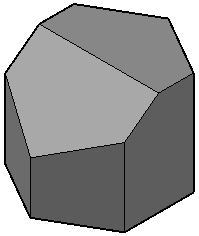
\includegraphics[scale=0.8]{jiejiao1.png}}\hspace{30pt}
\subfloat[]{\label{fig:jiejiao2}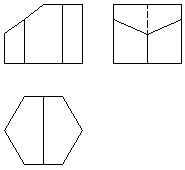
\includegraphics[scale=1]{jiejiao2.png}}
\caption{正六棱柱截交体}
\end{figure}
\subsubsection{棱锥截交体}
 图\ref{fig:jiejiao3}为正三边形棱柱截交体。该截交体的截交平面由平行于$H$面和垂直于$V$面的截交面构成,其三视图投影如图\ref{fig:jiejiao4}所示。
 \begin{figure}[htbp]
 \centering
\subfloat[]{\label{fig:jiejiao3}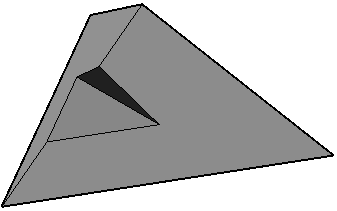
\includegraphics[scale=0.6]{jiejiao3.png}}\hspace{30pt}
\subfloat[]{\label{fig:jiejiao4}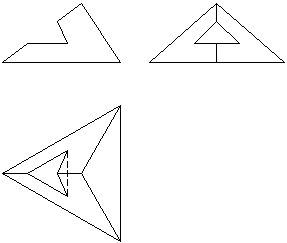
\includegraphics[scale=0.65]{jiejiao4.png}}
\caption{正六棱柱截交体}
\end{figure}
\subsubsection{圆柱截交体}
 \begin{figure}[htbp]
 \centering
\subfloat[]{\label{fig:jiejiao5}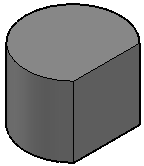
\includegraphics[scale=0.8]{jiejiao5.png}}\hspace{60pt}
\subfloat[]{\label{fig:jiejiao6}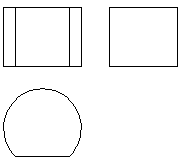
\includegraphics[scale=0.8]{jiejiao6.png}}\\
\subfloat[]{\label{fig:jiejiao7}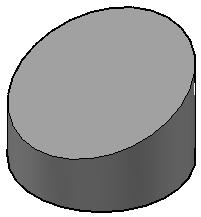
\includegraphics[scale=0.6]{jiejiao7.png}}\hspace{60pt}
\subfloat[]{\label{fig:jiejiao8}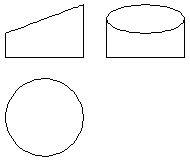
\includegraphics[scale=0.8]{jiejiao8.png}}\\
\subfloat[]{\label{fig:jiejiao9}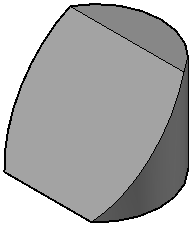
\includegraphics[scale=0.6]{jiejiao9.png}}\hspace{60pt}
\subfloat[]{\label{fig:jiejiao10}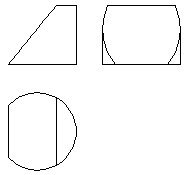
\includegraphics[scale=0.9]{jiejiao10.png}}
\caption{圆柱截交体}
\end{figure}
图\ref{fig:jiejiao5}为截交平面与轴线平,其截交线为一矩形,图\ref{fig:jiejiao6}是其三视图;图\ref{fig:jiejiao7}为截交面倾斜于轴线且不与上下表面相交,其截交线为一椭圆,图\ref{fig:jiejiao8}是其三视图;图\ref{fig:jiejiao9}为截交平面倾斜于轴线且与上下表面相交,其截交线为为复合图形,图\ref{fig:jiejiao10}是其三视图。
\clearpage
\subsubsection{圆锥截交体}
 \begin{figure}[htbp]
 \centering
\subfloat[]{\label{fig:jiejiao11}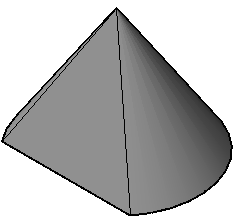
\includegraphics[scale=0.45]{jiejiao11.png}}\hspace{60pt}
\subfloat[]{\label{fig:jiejiao12}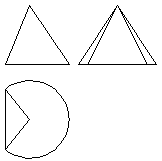
\includegraphics[scale=0.65]{jiejiao12.png}}\\
\subfloat[]{\label{fig:jiejiao13}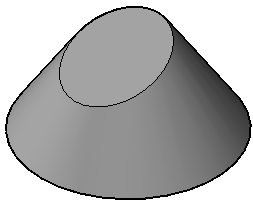
\includegraphics[scale=0.45]{jiejiao13.png}}\hspace{60pt}
\subfloat[]{\label{fig:jiejiao14}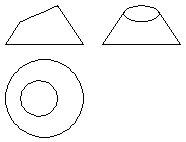
\includegraphics[scale=0.65]{jiejiao14.png}}\\
\subfloat[]{\label{fig:jiejiao15}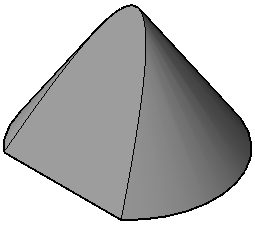
\includegraphics[scale=0.45]{jiejiao15.png}}\hspace{60pt}
\subfloat[]{\label{fig:jiejiao16}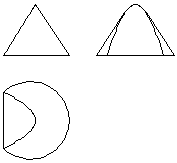
\includegraphics[scale=0.65]{jiejiao16.png}}\\
\subfloat[]{\label{fig:jiejiao17}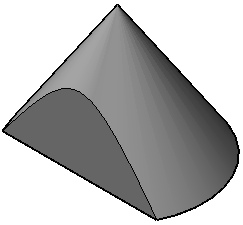
\includegraphics[scale=0.45]{jiejiao17.png}}\hspace{60pt}
\subfloat[]{\label{fig:jiejiao18}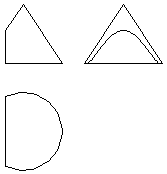
\includegraphics[scale=0.65]{jiejiao18.png}}
\caption{圆锥截交体}
\end{figure}
图\ref{fig:jiejiao11}为截交面通圆锥体锥顶,其截交线为三角形,图\ref{fig:jiejiao12}为其三视图;图\ref{fig:jiejiao13}为截面倾斜于轴线且倾斜角度大于锥角,其截交线为椭圆,图\ref{fig:jiejiao14}为其三视图;图\ref{fig:jiejiao15}为截面倾斜于轴线且倾斜角度等于锥角,其截交线为抛物线,图\ref{fig:jiejiao16}为其三视图;图\ref{fig:jiejiao17}为截面与轴线平行,其截交线为双曲线,图\ref{fig:jiejiao18}为其三视图。
\endinput
 